\chapter{Volume Average Method}
\label{ch:vans}

\section{Introduction}


\section{Derivation of VANS equations for 3D incompressible fluids}
\subsection{Definition of the averaging filter}

In the figure \ref{fig:rev} is an illustration of our porous problem; in the same figure we show all the main definition that we need to introduce in order to develop our mathematical approach.


\begin{figure}[H]
	\centering
	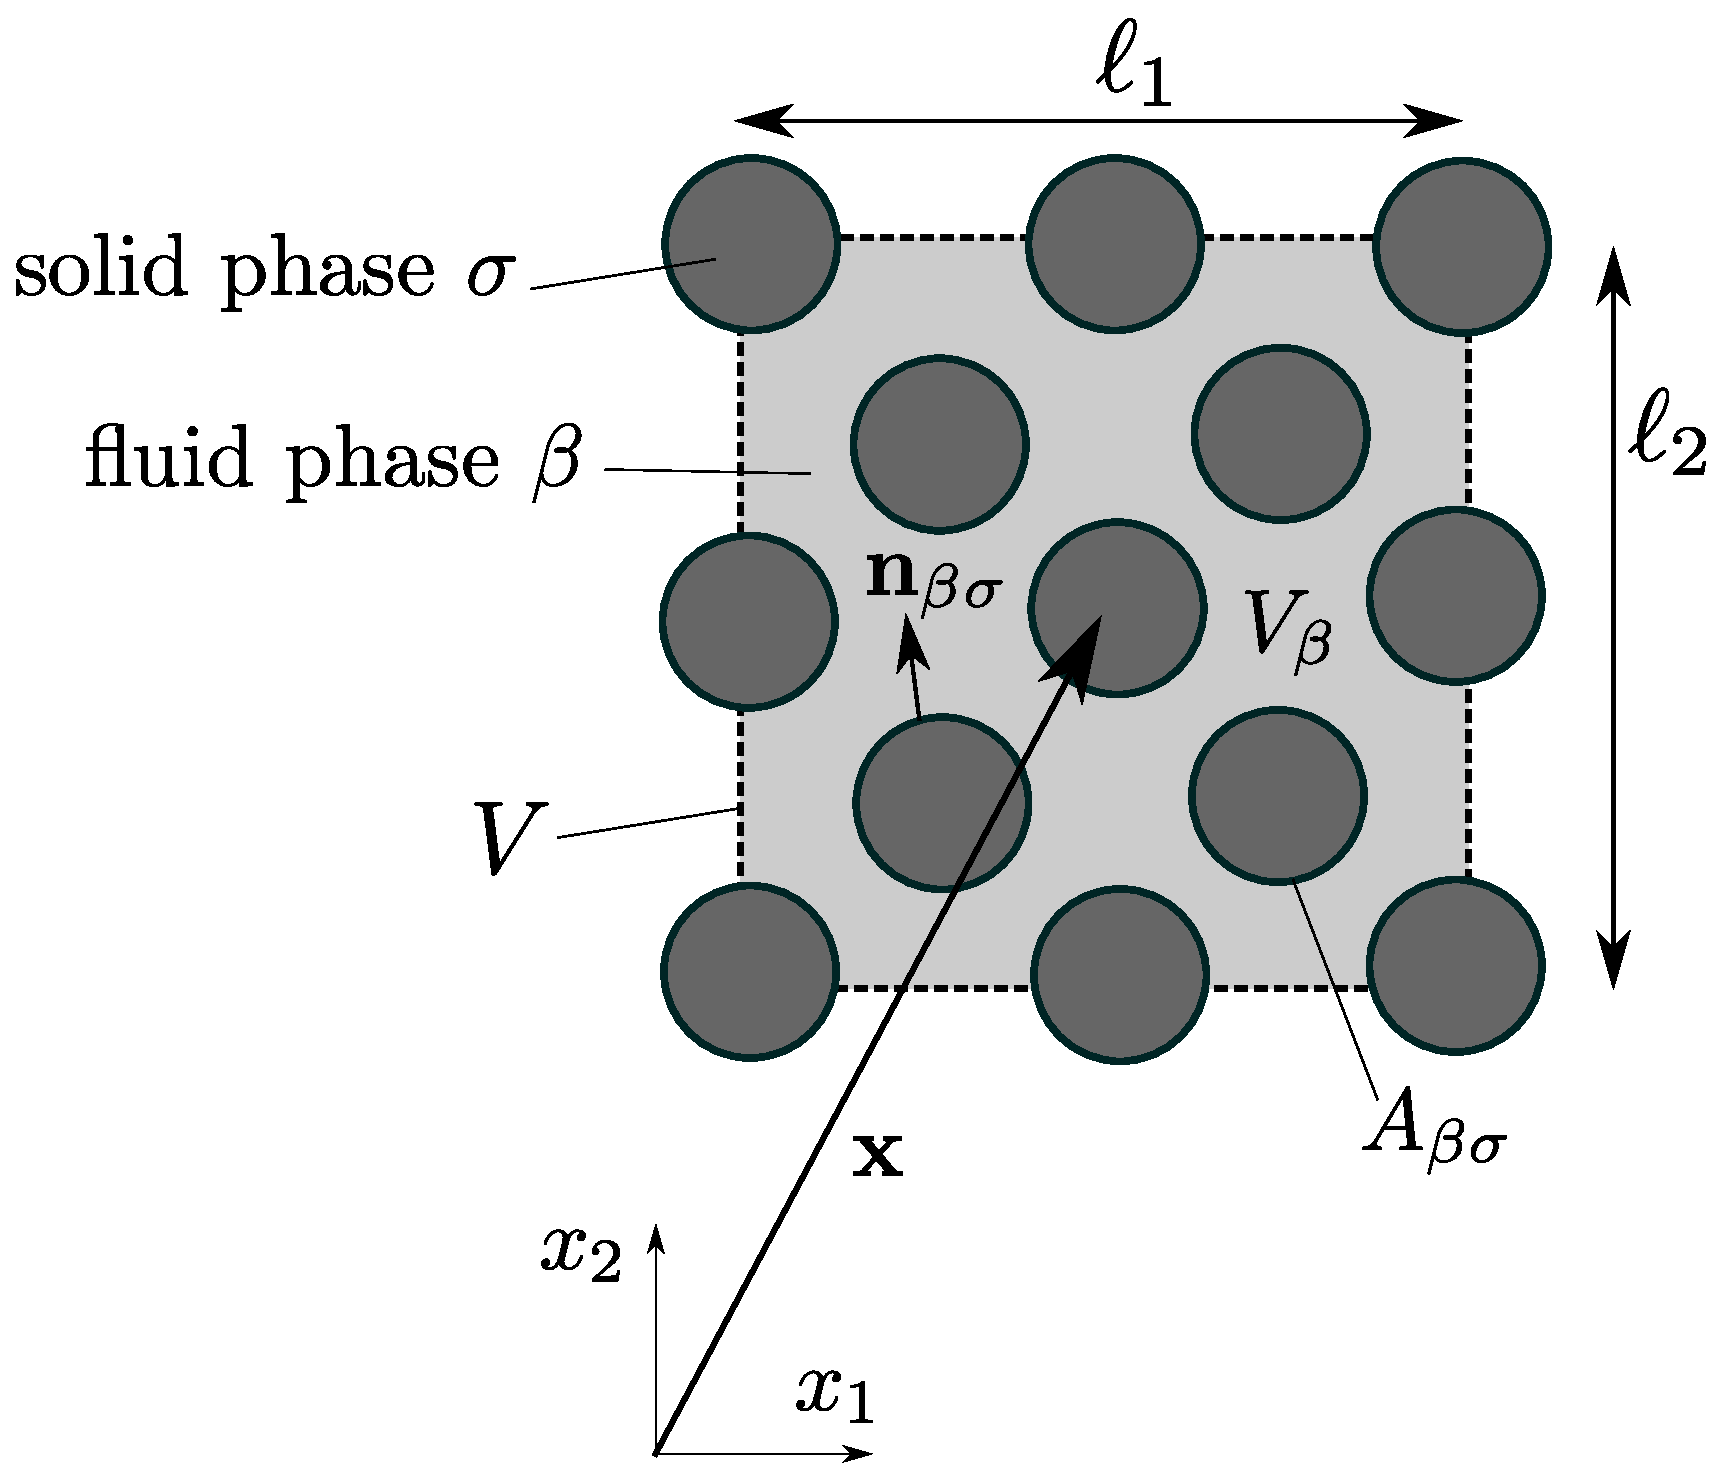
\includegraphics[width=0.8\linewidth]{chapter_4/figure/REV}
	\caption{Illustration of the REV concept.}
	\label{fig:rev}
\end{figure}


\begin{equation}
\meani{\psi_{\beta}}(\mathbf{X}, t) = \dfrac{1}{\volb} \int_{\volb} m(\mathbf{y}) \psi_{\beta}(\mathbf{x}-\mathbf{y}, t) d \volb.
\label{eq:avg_intrinsic}
\end{equation}


\begin{equation}
\meani{\psi_{\beta}}|_{\mathbf{x}} = \dfrac{1}{\volb} \int_{\volb(\mathbf{x})}  m(\mathbf{y}) \psi_{\beta}(\mathbf{x}-\mathbf{y}, t) d \volb.
\label{eq:avg_intrinsic_ext}
\end{equation}

\begin{equation}
\means{\psi_{\beta}} = \dfrac{1}{V} \int_{\volb} \psi_\beta (\mathbf{x}) d \volb.
\label{eq:avg_superficial}
\end{equation}


\begin{equation}
	\varepsilon = \dfrac{\volb}{V}
	\label{eq:porosity}
\end{equation}

\begin{equation}
	\means{\psi_{\beta}} =  \varepsilon \meani{\psi_{\beta}}
\end{equation}

\subsection{Theorems involving derivatives of spatial averaging}

\begin{theorem}[Averaging theorem Howes and Withaker, 1985]
\[	\means{\nabla \psi_{\beta}} = \nabla \means{\psi_{\beta}} + \dfrac{1}{V}\int_{A_{\beta \sigma}} \mathbf{n}_{\beta \sigma} \psi_{\beta} dA \]
\end{theorem}


\subsection{Length scale decomposition}

\begin{equation}
	\psi_{\beta} = \meani{\psi_{\beta}} + \tilde{\psi}_{\beta}
 \end{equation}

\subsection{Averaged continuity equations}


\begin{equation}
\nabla \cdot \vb = 0
\label{eq:cont}
\end{equation}

\subsection{Averaged momentum equations}


\begin{equation}
\dfrac{\partial \vb}{\partial t} + \vb \cdot \nabla \vb = -\frac{1}{\rho_{\beta}} \nabla \pb + \nub \nabla^2  \vb  + \mathbf{f}
\label{eq:mom}
\end{equation}




